% id: 12-43
% book: 베이직쎈 미적분1 · 01 함수의 극한
% section: 개념 05 함수의 극한값의 존재
% passage: 다음 극한을 조사하시오.
% figure: tikz:fig-12-43
% answer: 
% answer_source: 
% variant_level: 0 (원본 전사)
% 이 파일은 build.mjs 가 items.json 에서 만든다. 고칠 때는 items.json 을 고친다.
\smash{\raisebox{4.5mm}{\dmkichul{베이직쎈 미적분1 12쪽 43번}}}
\noindent\begin{minipage}[t]{0.58\linewidth}\vspace{0pt}\raggedright $\displaystyle\lim_{x\to 0}\dfrac{|x|}{x}$\end{minipage}\hfill\begin{minipage}[t]{0.4\linewidth}\vspace{0pt}\centering \resizebox{\ifdim\width>\linewidth\linewidth\else\width\fi}{!}{% 12-43(12쪽) — 43번 풀이 힌트의 그림 · y=|x|/x 의 그래프(x>0 에서 y=1, x<0 에서 y=-1 · 원점에서 끊긴 빈 점 · 다가가는 방향 화살표 네 개). 스캔 화질이 낮아 TikZ 로 다시 그림.
% 원문에 있는 것만: 빈 점 (0,1), (0,-1) · 라벨 1, -1, y=f(x), O, x, y · 접근 화살표. 눈금은 만들지 않는다.
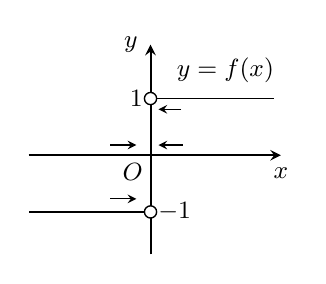
\begin{tikzpicture}[x=0.72cm, y=0.72cm, line width=0.6pt]
  \draw[->, >=stealth, line width=0.7pt] (-2.15,0) -- (2.3,0) node[below=1pt, font=\small] {$x$};
  \draw[->, >=stealth, line width=0.7pt] (0,-1.75) -- (0,1.95) node[left=1pt, font=\small] {$y$};
  \draw[line width=0.6pt] (0,1) -- (2.18,1);
  \draw[line width=0.6pt] (-2.14,-1) -- (0,-1);
  \draw[fill=white, line width=0.5pt] (0,1) circle (2.2pt);
  \draw[fill=white, line width=0.5pt] (0,-1) circle (2.2pt);
  \draw[->, >=stealth, line width=0.4pt] (0.54,0.81) -- (0.14,0.81);
  \draw[->, >=stealth, line width=0.4pt] (-0.71,-0.77) -- (-0.25,-0.77);
  \draw[->, >=stealth, line width=0.4pt] (-0.71,0.18) -- (-0.25,0.18);
  \draw[->, >=stealth, line width=0.4pt] (0.57,0.18) -- (0.14,0.18);
  \node[font=\small, inner sep=2.5pt, left] at (0,1) {$1$};
  \node[font=\small, inner sep=2.5pt, right] at (0,-1) {$-1$};
  \node[font=\small, inner sep=2.5pt, below left] at (0,0) {$\pt{O}$};
  \node[font=\small, inner sep=1pt] at (1.32,1.5) {$y=f(x)$};
\end{tikzpicture}
}\end{minipage}\par
\dmhint{$|x|=\begin{cases} x & (x\ge 0) \\ -x & (x<0) \end{cases}$이므로 $f(x)=\dfrac{|x|}{x}$로 놓으면\hfill{\footnotesize $f(x)$는 $x=0$에서 정의되지 않는다.}\\ $f(x)=\begin{cases} \blank & (x>0) \\ \blank & (x<0) \end{cases}$\\ $y=f(x)$의 그래프는 오른쪽 그림과 같으므로\\ $\displaystyle\lim_{x\to 0+} f(x)=\blank$,\\ $\displaystyle\lim_{x\to 0-} f(x)=\blank$\\ 따라서 $\displaystyle\lim_{x\to 0+} f(x)\ne\lim_{x\to 0-} f(x)$이므로\\ $\displaystyle\lim_{x\to 0} f(x)$, 즉 $\displaystyle\lim_{x\to 0}\dfrac{|x|}{x}$의 값은 \blank[6em].}
